\documentclass[a4paper]{article}

\usepackage{tikz}
\usetikzlibrary{positioning, arrows.meta, shapes, calc, fit}
\usepackage{float}
\usepackage{geometry}
\usepackage{xcolor}
\geometry{margin=1cm, landscape}

\begin{document}

\title{System Overview: Neuro-Symbolic Architecture (Runtime Injection)}
\author{}
\date{}
\maketitle

\section{Architecture Diagram}

This diagram illustrates the implemented **Neuro-Symbolic Architecture**. Unlike traditional "What-If" approaches that modify the BPMN model statically, this solution **intercepts the simulation engine at runtime**. It injects a "Neural Brain" (LSTM) for prediction and a "Symbolic Guard" (Rules) for validation directly into the decision-making process of the Discrete Event Simulator (Prosimos).

\begin{figure}[H]
  \centering
  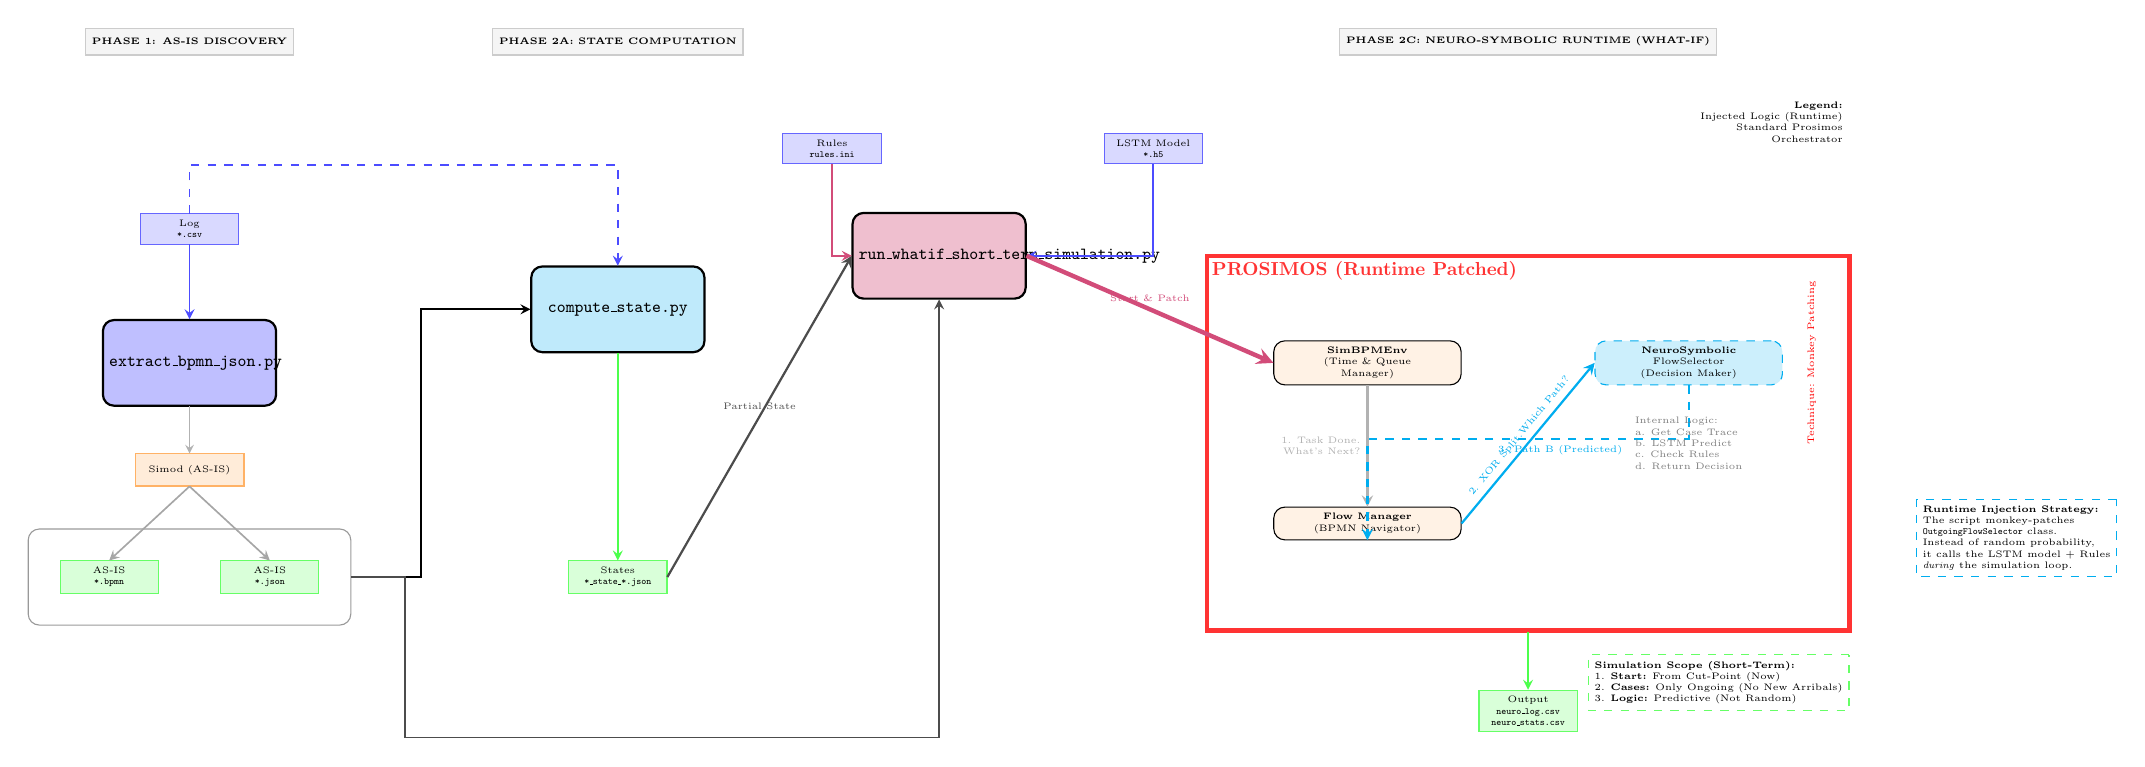
\begin{tikzpicture}[
    scale=0.68,
    transform shape,
    node distance=0.8cm and 1.5cm,
    script/.style={rectangle, rounded corners, draw=black, thick, 
                   minimum width=3.2cm, minimum height=1.6cm, 
                   text width=3cm, align=center, font=\small\bfseries},
    procstep/.style={rectangle, rounded corners, draw=black, fill=gray!10,
                 minimum width=2.5cm, minimum height=0.6cm,
                 text width=2.3cm, align=center, font=\tiny},
    input/.style={rectangle, draw=blue!60, fill=blue!15, 
                  minimum width=1.8cm, minimum height=0.5cm, 
                  text width=1.6cm, align=center, font=\tiny},
    output/.style={rectangle, draw=green!60, fill=green!15, 
                   minimum width=1.8cm, minimum height=0.5cm, 
                   text width=1.6cm, align=center, font=\tiny},
    config/.style={rectangle, draw=purple!60, fill=purple!15, 
                   minimum width=1.8cm, minimum height=0.5cm, 
                   text width=1.6cm, align=center, font=\tiny},
    tool/.style={rectangle, draw=orange!60, fill=orange!15,
                 minimum width=2cm, minimum height=0.6cm,
                 text width=1.8cm, align=center, font=\tiny},
    arrow/.style={->, >=stealth, semithick},
    phase/.style={rectangle, draw=gray!40, fill=gray!8, 
                  minimum width=3cm, minimum height=0.5cm, 
                  font=\tiny\bfseries, align=center},
    internal/.style={->, >=stealth, thin, gray!60}
  ]
    
    % Phase labels at top
    \node[phase] (phase1) at (-17, 10) {PHASE 1: AS-IS DISCOVERY};
    \node[phase] (phase2a) at (-9, 10) {PHASE 2A: STATE COMPUTATION};
    \node[phase] (phase2c) at (8, 10) {PHASE 2C: NEURO-SYMBOLIC RUNTIME (WHAT-IF)};
    
    % ========== PHASE 1: AS-IS MODEL ==========
    \node[input] (log) at (-17, 6.5) {Log\\\texttt{*.csv}};
    \node[script, fill=blue!25] (extract) at (-17, 4) {\texttt{extract\_bpmn\_json.py}};
    \node[tool] (simod1) at (-17, 2) {Simod (AS-IS)};
    \node[output] (bpmn-asis) at (-18.5, 0) {AS-IS\\\texttt{*.bpmn}};
    \node[output] (json-asis) at (-15.5, 0) {AS-IS\\\texttt{*.json}};
    \node[draw=gray!80, rounded corners, inner sep=0.4cm, fit=(bpmn-asis) (json-asis)] (simod-box) {};
    
    \draw[arrow, blue!70] (log.south) -- (extract.north);
    \draw[internal] (extract.south) -- (simod1.north);
    \draw[arrow, gray!70] (simod1.south) -- (bpmn-asis.north);
    \draw[arrow, gray!70] (simod1.south) -- (json-asis.north);
    
    % ========== PHASE 2A: STATE ==========
    \node[script, fill=cyan!25] (compute) at (-9, 5) {\texttt{compute\_state.py}};
    \node[output] (states) at (-9, 0) {States\\\texttt{*\_state\_*.json}};
    
    \draw[arrow, blue!70, dashed] (log.north) -- ++(0,0.9) -| (compute.north);
    \draw[arrow] (simod-box.east) -- ++(1.3,0) |- (compute.west);
    \draw[arrow, green!70] (compute.south) -- (states.north);

    % ========== PHASE 2C: NEURO-SYMBOLIC RUNTIME ==========
    
    % Orchestrator Script
    \node[script, fill=purple!25] (neuro-script) at (-3, 6) {
      \texttt{run\_whatif\_short\_term\_simulation.py}
    };
    
    % External Inputs for What-If
    \node[input] (rules) at (-5, 8) {Rules\\\texttt{rules.ini}};
    \node[input] (lstm) at (1, 8) {LSTM Model\\\texttt{*.h5}};
    
    \draw[arrow, purple!70] (rules.south) |- (neuro-script.west);
    \draw[arrow, blue!70] (lstm.south) |- (neuro-script.east);
    
    % Input from Phase 1 & 2A
    \draw[arrow, black!70, thick] (states.east) -- node[above, font=\tiny] {Partial State} (neuro-script.west);
    \draw[arrow, black!70] (simod-box.east) -- ++(1,0) -- ++(0, -3) -| (neuro-script); % AS-IS Model enters Prosimos directly
    
    % --- THE MONKEY-PATCHED ENGINE ---
    \node[rectangle, draw=red!80, ultra thick, fill=white, minimum width=12cm, minimum height=7cm] (engine-box) at (8, 2.5) {};
    \node[anchor=north west, font=\bfseries, text=red!80] at (engine-box.north west) {PROSIMOS (Runtime Patched)};
    
    % Components inside Prosimos
    \node[procstep, fill=orange!10, minimum width=3.5cm] (sim-env) at (5, 4) {\textbf{SimBPMEnv}\\(Time \& Queue Manager)};
    \node[procstep, fill=orange!10, minimum width=3.5cm] (flow-mgr) at (5, 1) {\textbf{Flow Manager}\\(BPMN Navigator)};
    
    % The INJECTED Components (Monkey-Patched)
    \node[procstep, fill=cyan!20, dashed, draw=cyan, minimum width=3.5cm] (injector) at (11, 4) {\textbf{NeuroSymbolic}\\FlowSelector\\(Decision Maker)};
    
    % Annotations for Injection
    \node[font=\tiny, text=red, rotate=90, anchor=south] at (13.5, 4) {Technique: Monkey Patching};
    
    % Wiring inside Engine (The Dialogue)
    \draw[internal, thick] (sim-env.south) -- node[left, font=\tiny, align=right] {1. Task Done.\\What's Next?} (flow-mgr.north);
    
    \draw[internal, thick, cyan] (flow-mgr.east) -- node[above, font=\tiny, text=cyan, sloped] {2. XOR Split.\\Which Path?} (injector.west);
    
    \draw[internal, thick, cyan, dashed] (injector.south) -- ++(0,-1) -| node[pos=0.2, below, font=\tiny, text=cyan] {3. Path B (Predicted)} (flow-mgr.south);
    
    % Logic inside Injector
    \node[font=\tiny, align=left, text=gray] at (11, 2.5) {
        Internal Logic:\\
        a. Get Case Trace\\
        b. LSTM Predict\\
        c. Check Rules\\
        d. Return Decision
    };
    
    % Script triggers Engine
    \draw[arrow, purple!70, ultra thick] (neuro-script.east) -- node[above, font=\tiny] {Start \& Patch} (sim-env.west);
    
    % Outputs
    \node[output] (out-neuro) at (8, -2.5) {Output\\\texttt{neuro\_log.csv}\\\texttt{neuro\_stats.csv}};
    \draw[arrow, green!70] (engine-box.south) -- (out-neuro.north);
    
    % LEGEND
    \node[anchor=north east, font=\tiny, align=right] at (14, 9) {
        \textbf{Legend:}\\
        \textcolor{cyan!80}{$\blacksquare$} Injected Logic (Runtime)\\
        \textcolor{orange!80}{$\blacksquare$} Standard Prosimos\\
        \textcolor{purple!80}{$\blacksquare$} Orchestrator
    };
    
    % Simulation Scope Explanation
    \node[rectangle, draw=green!60, dashed, fill=white, align=left, font=\tiny, anchor=south east] at (14, -2.5) {
        \textbf{Simulation Scope (Short-Term):}\\
        1. \textbf{Start:} From Cut-Point (Now)\\
        2. \textbf{Cases:} Only Ongoing (No New Arribals)\\
        3. \textbf{Logic:} Predictive (Not Random)
    };
    
    % Explain injection
    \node[rectangle, draw=cyan, dashed, fill=white, align=left, font=\tiny, anchor=south east] at (19, 0) {
        \textbf{Runtime Injection Strategy:}\\
        The script monkey-patches\\
        \texttt{OutgoingFlowSelector} class.\\
        Instead of random probability,\\
        it calls the LSTM model + Rules\\
        \textit{during} the simulation loop.
    };
    
  \end{tikzpicture}
  \caption{Neuro-Symbolic Runtime Architecture. Instead of generating synthetic data beforehand, we inject a \textbf{Neuro-Symbolic Flow Selector} directly into the Prosimos engine memory. The \texttt{run\_whatif\_short\_term\_simulation.py} script loads the AS-IS model, the LSTM brain, and the Declarative Rules. It then "patches" the simulation engine so that every XOR gateway decision is routed through the Neural Network (for prediction) and the Logic Monitor (for validation), strictly adhering to the Partial State from Phase 2A.}
  \label{fig:neuro-arch}
\end{figure}

\newpage

\section{Technical Deep Dive \& Defense}

This section details the internal mechanics of the Neuro-Symbolic engine, addressing key questions regarding its implementation and behavior.

\subsection{Core Components: Who Does What?}
The engine divides responsibilities between standard simulation mechanics and intelligent decision making:

\begin{itemize}
    \item \textbf{SimBPMEnv (Time \& Queue Manager):} The "Clock" of the simulation. It doesn't know \textit{how} to make decisions; it only knows \textit{when} events happen. It manages the event queue and advances simulation time. When a task finishes, it asks the Flow Manager "What comes next?".
    
    \item \textbf{Flow Manager (Structure Navigator):} The "Map" of the process. It holds the BPMN graph structure. It knows that after Task A comes an XOR gateway. But it doesn't know which path to take. In a standard simulation, it would roll a dice (probability). Here, it delegates to our injected component.
    
    \item \textbf{NeuroSymbolic FlowSelector (Decision Maker):} The "Brain". This is the injected class that replaces the random probability selector. It receives the query "We are at Gateway X, for Case Y. Where do we go?". It then runs the Neuro-Symbolic logic (LSTM + Rules) to return the optimal, valid path back to the Flow Manager.
\end{itemize}

\subsection{Core Mechanism: Runtime Injection (Monkey Patching)}
The system does \textbf{not} require rewriting the Prosimos library. Instead, it uses Python's dynamic capabilities ("Monkey Patching") to replace core components in memory just before execution:
\begin{itemize}
    \item \textbf{Target:} The \texttt{OutgoingFlowSelector} class in Prosimos, responsible for XOR gateway decisions.
    \item \textbf{Replacement:} It is swapped with \texttt{NeuroSymbolicFlowSelector}.
    \item \textbf{Effect:} The simulation engine continues to manage time, resources, and queues normally, but "outsource" routing decisions to our custom logic.
\end{itemize}

\subsection{Decision Logic: The "Hybrid Brain"}
Unlike standard simulation (Monte Carlo) which uses static probabilities (e.g., "50\% Left, 50\% Right"), this system makes \textbf{context-aware predictions}:
\begin{enumerate}
    \item \textbf{Context Retrieval:} When a case reaches a decision point, the engine extracts its full execution history (trace) from memory.
    \item \textbf{Neural Inference (LSTM):} This history is fed into the Deep Learning model, which predicts the most likely next activity based on learned patterns.
    \item \textbf{Symbolic Validation (Rules):} The prediction is checked against Declarative Rules (LTL). Example: \textit{"If 'Invoice Rejected', 'Pay' cannot happen"}.
    \item \textbf{Final Decision:} If valid, the path is taken. If invalid, the system falls back to the next best valid option, ensuring compliance.
\end{enumerate}

\subsection{Simulation Scope: Short-Term Specifics}
The simulation is strictly \textbf{Short-Term} and \textbf{Forward-Looking}:
\begin{itemize}
    \item \textbf{Start Point ($t_0$):} The simulation begins exactly at the Cut-Point timestamp provided by the Partial State. It does not simulate the past.
    \item \textbf{Case Population:} No new cases are generated ($Arrivals = 0$). The simulation only processes the specific cases that were "ongoing" (alive) at $t_0$.
    \item \textbf{Goal:} To predict the future trajectory of the \textit{current backlog} under the new declarative rules.
\end{itemize}

\end{document}
